\chapter{3-D Face Recognition Based on Ridge Images} In this
chapter, we present a method for 3-D face recognition from
frontal/near-frontal range images based on the ridge lines on the
surface of the face. As we discussed in chapter one, the surface
matching techniques suffer from computational complexity. In our
approach, a subset of points on the surface of the face are selected
using the principal curvature, $k_{max}$. These points show the
locations of the ridge points around the important facial regions on
the face, i.e., the eyes, the nose, and the mouth. Instead of
matching all the points on the surface of the face, the ridge points
are used for matching which leads to huge reduction of the
computational complexity while keeping the performance of the system
for face recognition promising. We compare the robust Hausdorff
distance versus the Iterative Closest Points (ICP) for matching the
ridge image of a given probe image to the ridge images of the facial
images in the gallery.

\section{3-D Face Matching Based on Ridge Images}
Figure \ref{fig_block_diagram} shows the block diagram of our
method. In the first step, because of noise and artifacts in the
range images, we use median filtering and low-pass filtering to
remove sharp spikes and smooth the images and then we use
interpolation to fill the gaps in the image. In the next step, we
roughly find the tip of the nose which is the closest point to the
scanner. Because the facial range images in the databases that we
work on are frontal/near-frontal, the claim that the tip of the nose
is the closest point to the scanner is valid. Then, we apply
template matching to localize the face region in the filtered range
data. Afterward, we use Gaussian curvature to label three feature
points, i.e., the inner corners of the two eyes and the accurate
position of the nose tip. We represent the range images by the
points on the 3-D surface of the face which have maximum principal
curvature, $k_{max}$, greater than a threshold. Therefore, each
range image is represented by ridge lines on the 3-D surface of the
face using a 3-D binary image, called ridge image. The details of
the preprocessing techniques and 3-D facial features labeling were
presented in Chapter three.

\begin{figure}[bp]
\begin{center}
\includegraphics
[scale = 0.5, angle = -90]{./chapters/Figures/ridge_general_bd.eps}
\caption{Block diagram of our system for 3-D face recognition from
range data.} \label{fig_block_diagram}
\end{center}
\end{figure}

For recognition, we use two different techniques for ridge image
matching: the robust Hausdorff distance and the Iterative Closest
Points (ICP). First, we apply similarity transformation (scale,
rotation and translation) to find the best pose that matches the
probe image with the gallery image. The three labeled feature points
plus an auxiliary point in the middle of the triangle formed by the
three labeled points are used to find the initial transformation
that aligns the probe ridge image to the test ridge image. The $x$
and $y$ values of the auxiliary point are the average value of the
$x$ and $y$ values of the other three points and $z$ value comes
from the range image. After initial alignment, for matching based on
robust Hausdorff distance, an iterative algorithm is applied to find
the optimum pose that results in the minimum Hausdorff distance. For
matching based on ICP, we utilized a fast variation of ICP to find
the best geometric alignment between a 3-D ridge probe image and a
given 3-D ridge gallery image and compute the Mean Square Error
(MSE) distance between the ridge points.

\section{Ridge Image} Our goal is to extract and use the points
lying on ridge lines as the feature points. These points correspond
to the extreme ridge points of the surface. In the literature
\cite{Anoshkina94}, the ridges are defined as the umbilic points at
which the $k_{max}$ attains a local positive maximum. An umbilic
point is a point on a surface where the principal curvatures are
equal and are non-zero (in the case of zero curvature, the point is
called a flat point.) Intuitively, ridges are the points that form
the drainage patterns and are called valleys when the ridges are
looked from the opposite side.

There are different approaches to locate the ridges \cite{Lopez99}
of a 3-D surface. One of the main approaches applies thresholding
the $k_{max}$ values which is used in this work. We threshold the
$k_{max}$ values to find these points. The suitable threshold is
obtained based on a small training set that is different from the
images in the gallery. The suitable threshold is selected such that
the highest recognition rate for that small training set is
achieved. Then, in our experiments the suitable threshold (a fixed
value) is used for creating the ridge images for all the facial
images in the databases under evaluation. Figure
\ref{fig_ridge_points} shows few examples of the ridge images
obtained by thresholding the $k_{max}$ values. These are 3-D binary
images that show the locations of the ridge lines on the surface of
the face. The lines on the boundary of the face are filtered out and
are not considered as feature points for recognition. To filter out
the points on the boundary of the face, we ignore the points on the
boundary of the matched template within a margin. In other words,
after localizing the face by template matching, the points that are
within a certain distance (for example 15 pixels) from the boundary
of the matched face template are excluded from the process of ridge
creation.

\begin{figure}[tbp]
\begin{center}
\epsfig{figure=./chapters/Figures/ridge_samples.eps, scale = 0.7,
angle = -90} \caption{Sample of ridge image extracted for different
subjects.} \label{fig_ridge_points}
\end{center}
\end{figure}

\subsection{Ridge Matching Using Robust Hausdorff Distance}
Huttenlocher \textit{et al.} originally proposed Hausdorff distance
(HD) \cite{huttenlocher93} as a measure for object matching in
computer vision. Unlike other shape matching methods, HD can be
calculated without knowing the exact correspondences of the points
in different sets. Modifications to the Hausdorff distance raise its
capability to handle not only noisy points, but also missing data
from occlusion and outliers \cite{huttenlocher99}.

Given two sets of points $\mathcal{A} = \{a_1, a_2, ...,
a_{N_\mathcal{A}}\}$ and $\mathcal{B} = \{b_1, b_2, ...,
b_{N_\mathcal{B}}\}$ of size $N_\mathcal{A}$ and $N_\mathcal{B}$,
respectively, the partial Hausdorff distance between the two sets of
points, $\mathcal{A}$ and $\mathcal{B}$, is defined as: \beq
H(\mathcal{A}, \mathcal{B}) = max(h_K(\mathcal{A},\mathcal{B}),
h_K(\mathcal{B},\mathcal{A}))\eeq where
$h_K(\mathcal{A},\mathcal{B})$ and $h_K(\mathcal{B},\mathcal{A})$
represent the directed distance between the two sets $\mathcal{A}$
and $\mathcal{B}$. The directed distances of the partial HD are
defined as: \beq h_K(\mathcal{A},\mathcal{B}) = K^{th}_{a\epsilon
\mathcal{A}} d_{\mathcal{B}}(a), ~~ h_K(\mathcal{B},\mathcal{A}) =
K^{th}_{b\epsilon \mathcal{B}} d_{\mathcal{A}}(b)\eeq where
$d_{\mathcal{B}}(a)$ represents the minimum distance (e.g. Euclidean
distance) value at point $a$ to the point set $\mathcal{B}$,
$d_{\mathcal{A}}(b)$ represents the minimum distance (e.g. Euclidean
distance) value at point $b$ to the point set $\mathcal{A}$,
$K^{th}_{a \epsilon \mathcal{A}}$ denotes the $K^{th}$ ranked value
of $d_\mathcal{B}(a)$, and $K^{th}_{b \epsilon \mathcal{B}}$ denotes
the $K^{th}$ ranked value of $d_\mathcal{A}(b)$.

After Huttenlocher \textit{et al.}'s original work, researchers have
proposed many different definitions and methods to realize directed
HD. Dubbisson and Jain revised the original HD and investigated the
performance of 24 different Hausdorrf distance measures based on
their behavior in the presence of noise \cite{dubisson94}. They
proposed the modified Haussdorff distance MHD. Sim \textit{et al.}
applied the robust statistic techniques of regression analysis to
the computation of the HD measures for object matching, resulting in
two robust HD measures: M-HD based on M-estimation and least trimmed
square-HD (LTS-HD) based on LTS \cite{sim99}. Based on the
experimental matching performance of these different HD measures,
robust LTS-HD based on the least trimmed square (LTS) measure
\cite{sim99} is adopted in our work. In the proposed LTS-HD
\cite{sim99}, the directed distance
$h_{LTS}(\mathcal{A},\mathcal{B})$ is defined by a linear
combination of order statistics: \beq \label{eq_lts_HD}h_{LTS} =
\frac{1}{H}\sum_{i=1}^H d_\mathcal{B}(a)_{(i)} \eeq where $H$
denotes $h \times N_\mathcal{A}$ ( $0 \leq h \leq\ 1$) as in the
partial $HD$ case, and $d_\mathcal{B}(x)_{(i)}$ represents the
$i^{th}$ distance value in the sorted sequence
$d_\mathcal{B}(x)_{(1)} \leq d_\mathcal{B}(x)_{(2)} \leq \dots \leq
d_\mathcal{B}(x)_{(N_\mathcal{A})}$. The measure
$h_{LTS}(\mathcal{A},\mathcal{B})$ is calculated by eliminating the
large distance values and only keeping the $h$ fraction of the
minimum distances. In our experiments, the value of $h$ that
resulted in the best recognition rate was $0.8$.

In our case, the calculation of LTS-HD is between the two point sets
of two 3-D binary images, one is the ridge image of the test face
image and the other is the ridge image of a gallery face image. The
process of finding the best pose between a probe ridge image and a
gallery ridge image can be formulated as follows:

\beq \label{eq_optimization_2} \arg \min_{\alpha, \beta, \gamma,
t_x, t_y, t_z, s} h_{LTS}(Tr(\mathcal{A}), \mathcal{B}) \eeq where
$\textstyle\small{Tr = \left[\begin{array}{lr}sR &~ T\\
0^t &~ 1 \end{array}\right]}$ is a 3-D similarity transformation, s
is a scale factor, \\
$\textstyle{T = [t_x~t_y~t_z]'}$ is the 3-D translation, and $R$ is
a 3-D rotation matrix with $\alpha, \beta,$ and $\gamma$ as roll,
pith, and yaw rotation angels.

The process of finding the optimum pose between a probe ridge image
and a gallery ridge image is achieved by an iterative approach as
shown in table \ref{fig_Hausdorff_iterative}.

\begin{table}
\begin{tabular}{|p{5.7in}|}
\hline
\\

\textbf{(1)} Set $\hat{h}_{LTS} := +\infty$, and $t := 0$
\\
\textbf{(2)} Initially align the 3-D ridge image of the test image
$P$, i.e. translate, rotate and scale, to the gallery image $P'$, by
using the three labeled feature points and the auxiliary point. This
similarity transformation is calculated by procrustes analysis
\cite{procrustes}.
\\
\textbf{(3)} Set $Success := 0$
\\
\textbf{(4)} Place the aligned probe ridge image, $T(P)$, over the
gallery ridge image. For all the points in the aligned probe image,
find the distance to the closest point in the gallery image, $P'$,
using: \beq D_{P'}(x) = min_{y \in P'}||x - y||\eeq where the
$||.||$ denotes the $L2$ norm.
\\
\textbf{(5)} Sort the minimum calculated distances and then
calculate the robust Hausdorff distance, $h_{LTS}$, using Eq.
\ref{eq_lts_HD}.
\\
\textbf{(6)} If $(h_{LTS} <= \hat{h}_{LTS})$, set the following items:\\
$       \hat{h}_{LTS} := h_{LTS}$\\
$       t := t + 1$\\
$       Success := 1$
\\
\textbf{(7)} Change the parameters  i.e., translation, rotation, and
scale, of the similarity transformation based on the optimization
technique. For example, direct search in the simplex method.
\\
\textbf{(8)} If $Success = 1$ $AND$ $(t < Max\_Iterations)$ goto 3.
\\
\textbf{(9)} Return $h_{LTS}$.
\\
\hline
\end{tabular}
\caption{Iterative algorithm to find the optimum pose in Hausdorff
distance matching.} \label{fig_Hausdorff_iterative}
\end{table}

We used the Matlab optimization toolbox, i.e., \textit{fminsearch}
Matlab function, to solve this problem. The \textit{fminsearch} uses
the simplex search method of \cite{Lagarias98}. This is a direct
search method that does not use numerical or analytic gradients.

This procedure is repeated to find the matching distance between a
probe image and all the images in the gallery. The gallery face
image that results in the minimum matching distance, is considered
the best match.

\subsection{Ridge Matching Using Iterative Closest Points}
The ICP algorithm is widely used for geometric alignment of 3-D
models when an initial estimate of the relative pose is known. Many
variants of ICP have been proposed, where the differences are in the
phases of selecting, matching the feature points, and/or the
minimization strategy. In this work, we use a fast ICP variant
\cite{Rusinkiewicz_01}. Instead of using random sampling of the
feature points as in \cite{Rusinkiewicz_01}, we use all the feature
points in the 3-D ridge image in the matching process. Although
\textit{random sampling of the points} speeds up the matching
process, it has a adverse effect on the accuracy of the final
results. The details of the ICP algorithm is presented in Appendix
B.

For the initial alignment of a probe 3-D binary ridge image to the
3-D ridge images in gallery, the three labeled feature points, i.e.,
the two inner corners of the eyes and the tip of the nose and an
auxiliary point are utilized. Procrustes analysis \cite{procrustes}
is then used to estimate the parameters of the similarity
transformation (scale, rotation, and translation.) After the initial
alignment, we use the aforementioned ICP algorithm to finely align a
3-D ridge probe image with a given 3-D ridge gallery image and
compute the Mean Square Error (MSE) between the points. The smaller
the MSE the closer the probe image to the gallery image.

\subsection{Computational Complexity of Ridge Matching}
Compared to other 3-D matching approaches for face recognition such
as \cite{lu06,russ05,chang05}, i.e., the second category in our
classification, our approach is faster and requires less
computations. This reduction in computations is due to the fact that
we only deal with the ridge lines around the important facial
regions on the face, i.e., the eyes, the nose, and the mouth and
ignore the surface patches on the face during the matching process.
In other words, instead of matching the entire surface of two faces
(a probe image and a gallery image), we only match the ridge lines
on the face that are detected based on the principal curvature. In
this work, the number of the points in the ridge images that
represent the lines around the facial regions are $14\% \pm 2\%$ of
the total number of points that cover the face. The computational
complexity for both the robust Hausdorff distance and the ICP is
$O(PQ)$ with Euclidean distance calculations as the elementary
operations, where $P$ and $Q$ are the number of the points in the
probe and the gallery. By employing the K-D tree for searching the
closest points, the computational complexity is reduced to
$O(log(P))$. So, by using the ridge lines, only fraction of the
points on the surface of the face are used for face recognition. If
we assume that the ridge points are only a fraction, i.e., $\rho <
1$, of the entire points on face surface, e.g., $0.14 \pm 0.02$ in
our work, then the computational complexity reduces to
$\rho^{2}O(PQ)$ for the regular scheme and to $O(log(P) -
log(1/\rho))$ for the accelerated scheme. This means that by using
the ridge points, the computational complexity of matching is
reduced two orders of magnitude.

\section{Experiments and Results} \label{experiments} We use the
Gavab database \cite{moreno04} and the FRGC V2.0 \cite{FRGC2005} 3-D
face databases for our experiments. In the following subsections we
review these two databases and present our experiments and results.

\subsection{Experiments on Gavab Database} As described in Section
3.4, the Gavab database contains range images of 61 subjects. In our
experiments, we used the two neutral frontal images (the $1^{st}$
and the $2^{nd}$ captures), the two neutral looking up and down
images (the $5^{th}$ and the $6^{th}$ captures), the frontal images
with smile expression (the $7^{th}$ capture), the frontal images
with laughing expression (the $8^{th}$ capture), and a frontal image
with random gesture (the $9^{th}$ capture). The images in the
$2^{nd}$ capture are used as gallery images and the images in the
$1^{st}, 3^{rd}$, $4^{th}$, and $7-9^{th}$ captures are used as the
probe images for recognition.

Figure \ref{fig_sample_preprocessing} shows three samples of the
original images in the Gavab database, results of noise removal and
interpolation, face localization, feature points labeling, and ridge
images.

\begin{figure}[tbp]
\begin{center}
\epsfig{figure=./chapters/figures/Gavab_samples.eps, scale = 0.6,
angle = -90} \caption{Samples of range images in the gallery and the
results of preprocessing (a) Original range images, (b) Noise
removal and interpolation, (c) Face localization and three feature
points labeling, (d) Ridge images} \label{fig_sample_preprocessing}
\end{center}
\end{figure}
%%%%%%
For recognition, we compared between the robust Hausdorff distance
and the ICP techniques. Table \ref{table_results_GavabDB} presents
the results of the experiments. For neutral frontal images, only
four subjects out of 61 subjects were not identified by both
algorithms (93.5\% rank-one identification rate). In another
experiment, we projected the frontal ridge images to 2-D (ignoring
the $3^{rd}$ dimension) and the recognition process was tested. By
ignoring the $3^{rd}$ dimension, we obtained rank-one identification
rate of 82.0\% and 86.9\% using robust Hausdorff distance and ICP,
respectively. This result supports the opinion that 3-D data has
more potential for face recognition than 2-D data.

For faces with expressions, we considered only the upper part of the
face, i.e., the 3-D ridge lines around the eyes and the nose, for
recognition and excluded the lower part of the face, i.e., the
mouth, which is affected by the expression. We achieved a
recognition rate of 83.6\% using the ICP technique and 82.0\% using
the robust Hausdorff distance for the smiling expression.

Furthermore, we evaluated the performance of our approach for
recognition of facial images with pose (looking up/down) based on
both the ICP and the robust Hausdorff distance techniques. The
recognition rates for the facial images with the looking up (down)
pose are 88.6\% (85.3\%) and 75.4\% (70.5\%) using the ICP technique
and the robust Hausdorff distance, respectively.

\begin{table}
\centering
\begin{tabular}{|c|c|c|}
 \hline
  Facial Expression & \multicolumn{2}{c|}{$1^{st}$ Rank Recognition (\%)}\\
  \cline{2-3}
  &Robust H.D. & ICP\\
  \hline \hline
  Neutral (3-D) & 93.5 & 95.0\\
%  Neutral (2-D) & 82.0 & 86.9\\
  Smiling (3-D) & 82.0 & 83.6\\
  Laughing (3-D) & 73.8 & 68.9\\
  Random Gesture (3-D) & 63.4 & 63.4\\
  Looking Up (3-D) & 75.4 & 88.6\\
  Looking Down (3-D) & 70.5 & 85.3\\
  \hline
\end{tabular}
\caption{Results of first-ranked recognition rate on the Gavab face
database using range data.}\label{table_results_GavabDB}
\end{table}

Figure \ref{fig_cmc_gavabDB} and \ref{fig_roc_gavabDB} show the
performance of the system in term of Cumulative Match Characteristic
(CMC) curve and Receiver Operating Characteristic (ROC),
respectively, for the neutral versus neutral frontal facial images
using the ICP and the robust Hausdorff distance matching techniques.
Our experiments show that the performance of the ICP is better than
the robust Hausdorff distance for matching (except for the laughing
expression.)
%%%%%%%%%%%%%%

\begin{figure}[tbp]
\begin{center}
\epsfig{figure=./chapters/figures/cmc_gavabDB.eps, scale = 0.6}
\caption{CMC curves for frontal neutral images in Gavab database
based on ridge images matched using the ICP and Hausdorff distance
techniques.} \label{fig_cmc_gavabDB}
\end{center}
\end{figure}

\begin{figure}[tbp]
\begin{center}
\epsfig{figure=./chapters/figures/roc_gavabDB.eps, scale = 0.6}
\caption{ROC curves for frontal neutral images in Gavab database
based on ridge images matched using the ICP and Hausdorff distance
techniques.} \label{fig_roc_gavabDB}
\end{center}
\end{figure}

We compared our algorithm with three different approaches for 3-D
face recognition that were presented by Moreno \textit{et al.} in
\cite{Moreno03, Moreno05_1, Moreno05_2} based on the Gavab dataset.
In \cite{Moreno03}, they segmented the range images into isolated
subregions using the mean and the Gaussian curvatures. Then, they
extracted 86 descriptors such as the areas, the distances, the
angles, and the average curvatures of the subregions. They selected
35 best features and utilized them for face recognition based on the
minimum Euclidean distance classifier. They achieved a first ranked
recognition rate of 78.0\% for neutral frontal images and 62\% for
images with smile expression (only 60 subjects out of 61 from the
database were utilized). In \cite{Moreno05_1}, they selected a set
of 30 features out the 86 features and obtained recognition rates of
82.0\% and 90.16\%, when the images are frontal views with neutral
expression using Principal Component Analysis (PCA) and Support
Vector Machines (SVM), respectively. The recognition rates decreased
to 76.2\% and 77.9\%, using PCA and SVM matching schemes,
respectively, when using probe images with expressions and slight
face rotation. In \cite{Moreno05_2}, the authors represented the
face using 3-D voxels. Experiments were performed on both images
with neutral expression and images with either pose variations or
facial expressions. The best recognition rate that they achieved was
90.16\% for the images with neutral expression and 77.9\% for the
images with pose and facial expressions. In addition Ansari
\cite{Nasser07_thesis} applied a 3-D mesh modeling technique to
represent the data in Gavab database and used Euclidean distance and
voting for comparing 3-D meshes. As a result he achieved 90.16\%
Table \ref{tab_comparing_results_gavabDB} summaries their results as
well as ours. As the results show, our method based on ridge images
and the ICP technique for matching has a better recognition
performance for images with neutral expression, with expressions,
and with pose variations.
\begin{table}{\scriptsize \setstretch{0.75}}
\begin{center}
\begin{tabular}{|l|m{.82in}|m{0.75in}|l|} \hline
\textbf{Approach} & \textbf{Neutral-Neutral}\% & \textbf{Neutral-Pose/Expr.} \% & \textbf{Technique}\\
\hline \hline Moreno \etal\cite{Moreno03} & \centering 78.0 &
\centering 62.0 & 35 features(e.g., areas of subregions) \\ \hline
Moreno \etal\cite{Moreno05_1} & & & \\
& \centering 82.0 & \centering 76.2 & 30 features and PCA \\
& \centering 90.16 & \centering 77.9 & 30 features and SVM \\ \hline
Moreno \etal\cite{Moreno05_2} & \centering 90.16 & \centering 77.9 &
3-D volxels
\\ \hline
Ansari \cite{Nasser07_thesis} & \centering 90.16 & \centering - &
3-D Mesh
\\ \hline
\textbf{Our results} & \centering 93.5 & \centering 75.4/82.0 & Robust Hausdorff distance \\
& \centering 95.0 & \centering 88.6/83.6 & Iterative Closest Points \\
\hline
\end{tabular}
\end{center}
\caption{Comparing the results by Moreno \etal \cite{Moreno03,
Moreno05_1, Moreno05_2} and Ansari \cite{Nasser07_thesis} on Gavab
database and our work.} \label{tab_comparing_results_gavabDB}
\end{table}

\subsection{Experiments on FRGC V2.0 Face Database}
The FRGC V2.0 database \cite{FRGC2005} consists of 50,000 recordings
divided into training and validation partitions. The training
partition is designed for training algorithms and the validation
partition is for assessing the performance of a system in a
laboratory setting. FRGC V2.0 consists of six experiments, where the
third experiment measures the performance of 3-D face recognition.
In the third experiment, the gallery and probe data sets consist of
both range and texture images for each subject. The 3-D images were
acquired by a Minolta Vivid 900/910 series sensor. There are 4007
pairs of images (range and texture) for 466 subjects in the
validation set. The set contains images from 1 to 22 sessions per
subject, including images with neutral expression and images with
other expressions. 370 subjects have at least two images with
neutral expression and 432 subjects have at least one neutral image.
Figure \ref{fig_FRGC_samples} shows few samples of range images
along with the range data for different subjects in the FRGC V2.0
database.
\begin{figure}[tbp]
\begin{center}
  \includegraphics[scale = 0.75]{./chapters/Figures/frgc_samples.eps}\\
  \caption{Samples of facial images in the FRGC V2.0 database (texture, range, and extracted ridge images.)}
  \label{fig_FRGC_samples}
\end{center}
\end{figure}

We investigated the performance of our algorithm on the neutral 3-D
face images of the FRGC V2.0 database. First, we compared the
performance of the robust Hausdorff distance and the ICP technique
for matching the ridge images. There are 370 subjects that have at
least two neutral images captured in different sessions. For some of
the subjects, there are more than two captured neutral images with a
time laps of one week between them. We chose the two farthest
captured images for each subject and considered the oldest one as
the gallery and the most recent captured as the probe. The result of
rank-one identification using the robust Hausdorff distance on this
selected dataset is 41.62\% while the result of the ICP technique
for matching is 91.8\%. This means that the ICP based matching
approach not only gives the best performance, but also it is robust
with the increase in the size of the database. To remind the
readers, for a small size database such as Gavab, the performance of
the Hausdorff matching and the ICP matching were comparable (ICP was
slightly better.) This conclusion made by Yan and Bowyer in
\cite{Yan05}, where they compared ICP and Hausdorff for ear surface
matching: The ICP outperforms the Hausdorff distance for shape
matching.

\begin{figure}[tbp]
\begin{center}
\epsfig{figure=./chapters/figures/cmc_frgc.eps, scale = 0.6}
\caption{CMC curve for 370 subjects in the FRGC V2.0 database based
on ridge images matched with the ICP and Hausdorff techniques.}
\label{fig_cmc_frgc}
\end{center}
\end{figure}

\subsection{Comparison Between Recognition Using the Ridge Points, Random set of Points, and Entire Face Surface}
In order to justify that the ridge points are the important points
on the face for 3-D face matching, we experimented with 3-D face
recognition using random selection of the points from the entire
surface of the face and used the ICP method for matching. A set of
random points was selected from the range images such that the $x$
and $y$ coordinates are randomly selected using a random generator
with uniform distribution and the $z$ value of each point comes from
the existing depth values of the probe and the gallery image. The
number of the random points is equal to the average number of the
ridge points in the ridge image. Then, these random points are used
for matching based on the ICP technique. In addition we used all the
points on the face surface for matching based on the ICP technique.
The results of these experiments are summarized in table
\ref{tab_random_points} for the data GavabDB and FRGC V2.0.

\begin{table}
\begin{center}
\begin{tabular}{|c|c|c|c|}
 \hline
 Database&Ridge Points&Random Points&Complete Surface\\
\hline \hline
Gavab (61 subjects)&95.0&67.2& 95.0\\
FRGC V2.0 (370 subjects)&91.8&10.0&93.7\\
\hline
\end{tabular} \caption{Comparison between the ridge points, random points selection, and entire surface
based on the ICP matching technique; Results are in term of rank-one
identification rate (\%).}\label{tab_random_points}
\end{center}
\end{table}

The result of our experiment shows that the ridge points are robust
for 3-D face recognition versus random point selection for matching.
Specially, when the size of the database is large enough (370
subjects in FRGC V2.0), the performance of matching based on random
points selection is very low (10\% for the FRGC V2.0 dataset.)
Compared to the matching scheme using all the surface points, as
long as the size of the database is small, the ridge points and the
entire points on the surface of the face have the same performance.
With the increase in the size of the database, the recognition rate
does not drop significantly (91.8\% compared to 93.7\% on the
FRGC2.0 dataset.) In conclusion, there is a tradeoff between the
performance and computational complexity in shape matching and our
experiments show that ridge points are very promising in surface
matching. In other words, ridge points have good performance rate
while reducing the computational complexity of matching two orders
of magnitude.

\subsection{More Results on FRGC V2.0} In another experiment, we evaluated the capability of the
ridge images for face verification on FRGC V2.0 face database. Since
ICP has a better performance than robust HD technique for matching,
only the ICP technique is used in the rest of our experiments.
Figure \ref{fig_results_Neutral_ROC} shows the result of the
verification experiment for the neutral facial images (total of 2365
facial images for 432 individual subjects). The results are
presented using an ROC curve. As the ROC curve shows the performance
of 3-D face recognition based on ridge images and the ICP technique
for matching is 88.5\% verification at 0.1\% False Acceptance Rate
(FAR).
\begin{figure}[tbp]
\begin{center}
  \includegraphics[scale = 0.5]{./chapters/Figures/results_3D_ICP_FRGC.eps}\\
  \caption{ROC curve for the neutral faces versus neutral in FRGC2.0 database (total of 2365 facial
images for 432 individual subjects); ICP technique is used for
matching the ridge images.}\label{fig_results_Neutral_ROC}
\end{center}
\end{figure}
Table \ref{table_ROC_3-D} breaks down the results of the 3-D for
verification at 0.1\% FAR in terms of three different ROCs. In ROC I
all the data are within the semesters (Fall 2003 and Spring 2004),
in ROC II the data are within the year, and in ROC III the images
are between the semesters (see Figure \ref{fig_ROC_detail}). This
means that the experiment that produced ROC III is the toughest
experiment in term of time laps between the images. The table
represents the results of verification for neutral v.s. neutral
images in FRGC V2.0 dataset (2365 images of 432 subjects). The last
column of the table shows the results of the FRGC baseline for the
three ROCs. The baseline algorithm for the 3-D scans in FRGC
consists of applying PCA on the shape and texture channels
separately and then fusing the results. Compared to the FRGC
baseline, our approach has a better performance. Furthermore,
comparison between our results in the three ROCs, shows that the
performance of our system does not drop significantly under the
effect of aging and time laps between the capturing sessions. This
validates our claim that the ridge lines have great potential for
face recognition under the effect of aging.
\begin{table}{\setstretch{1.5}}
\begin{center}
\begin{tabular}{|c|c|c|}
 \hline
\textbf{Neutral}& 3-D (\%)& FRGC Baseline (\%)\\
\hline \hline
ROC I &90.69&90.00\\
ROC II &88.5&86.01\\
ROC III &85.75&81.58\\
\hline
\end{tabular} \caption{Verification rates (\%) at 0.1\% FAR for the ROC I, II, and III of the neutral v.s. neutral
images.}\label{table_ROC_3-D}
\end{center}
\end{table}

\begin{figure}[tbp]
\begin{center}
  \includegraphics[scale = 0.5]{./chapters/Figures/ROC_details_III.eps}\\
  \caption{ROC I: the data are within the semesters. ROC II: the data are within
the year. ROC III: the images are between the
semesters.}\label{fig_ROC_detail}
\end{center}
\end{figure}

\section{Summary}
In this chapter, we have presented an approach for 3-D face
recognition from frontal range data based on the ridge lines on the
face surface. We have used the principal curvature, $k_{max}$, to
represent the face image as a 3-D binary image called ridge image.
The ridge image shows the locations of the ridge points around the
important facial regions on the face, i.e., the eyes, the nose, and
the mouth. We have utilized the robust Hausdorff distance and the
Iterative Closest Points (ICP) for matching the ridge image of a
given probe image to the ridge images of the facial images in the
gallery. To test the performance of our approach for 3-D face
recognition, we have performed experiments on GavabDB face database
(a small size database) and Face Recognition Grand Challenge V2.0 (a
large size database). The results of the experiments have shown that
the ridge lines have great capability for 3-D face recognition. In
addition, we have found that as long as the size of the database is
small, the performance of the ICP based matching and the robust
Hausdorff matching are comparable. But, when the size of the
database increases, ICP based matching outperforms the robust
Hausdorff matching technique.
